% !TeX root = ../main.tex

%\section{Killer Whale Case Study}

\subsection{Data Collection and Preprocessing}

To apply this methodology to real-world data, the CarHHMM was used to analyze dive data from a killer whale off the coast of British Columbia, Canada. The data was collected on September 2, 2019 from 12:49 pm to 6:06 pm and consists of depth and acceleration in three orthogonal directions. Observations were collected at a rate of 50 hertz. Tagging the killer whale caused anomalous behavior before 1:20 pm and after 6:00 pm, so observations in this time range were ignored. In addition, the tagging technology dropped data between 2:25pm and 2:37pm as well as between 4:07 and 5:07 pm, so any partially observed data within this time range were ignored as well. A killer whale ``dive" is considered to be any continuous chunk of data that occurs below 0.5 meters in depth and lasts for at least 10 seconds. Accelerometer and depth data were smoothed by taking a moving average with a window of 1/10th of a second. Data preprocessing was done in part with the \textit{divebomb} package in Python \cite{Nunes:2018}. After preprocessing the raw data, a total of 267 dives were observed. A plot of the processed data for all dives and a collection of five selected dive can be seen in figures \ref{fig:data} and \ref{fig:data_one_dive}, respectively.

\begin{figure}[h!]
	\centering
	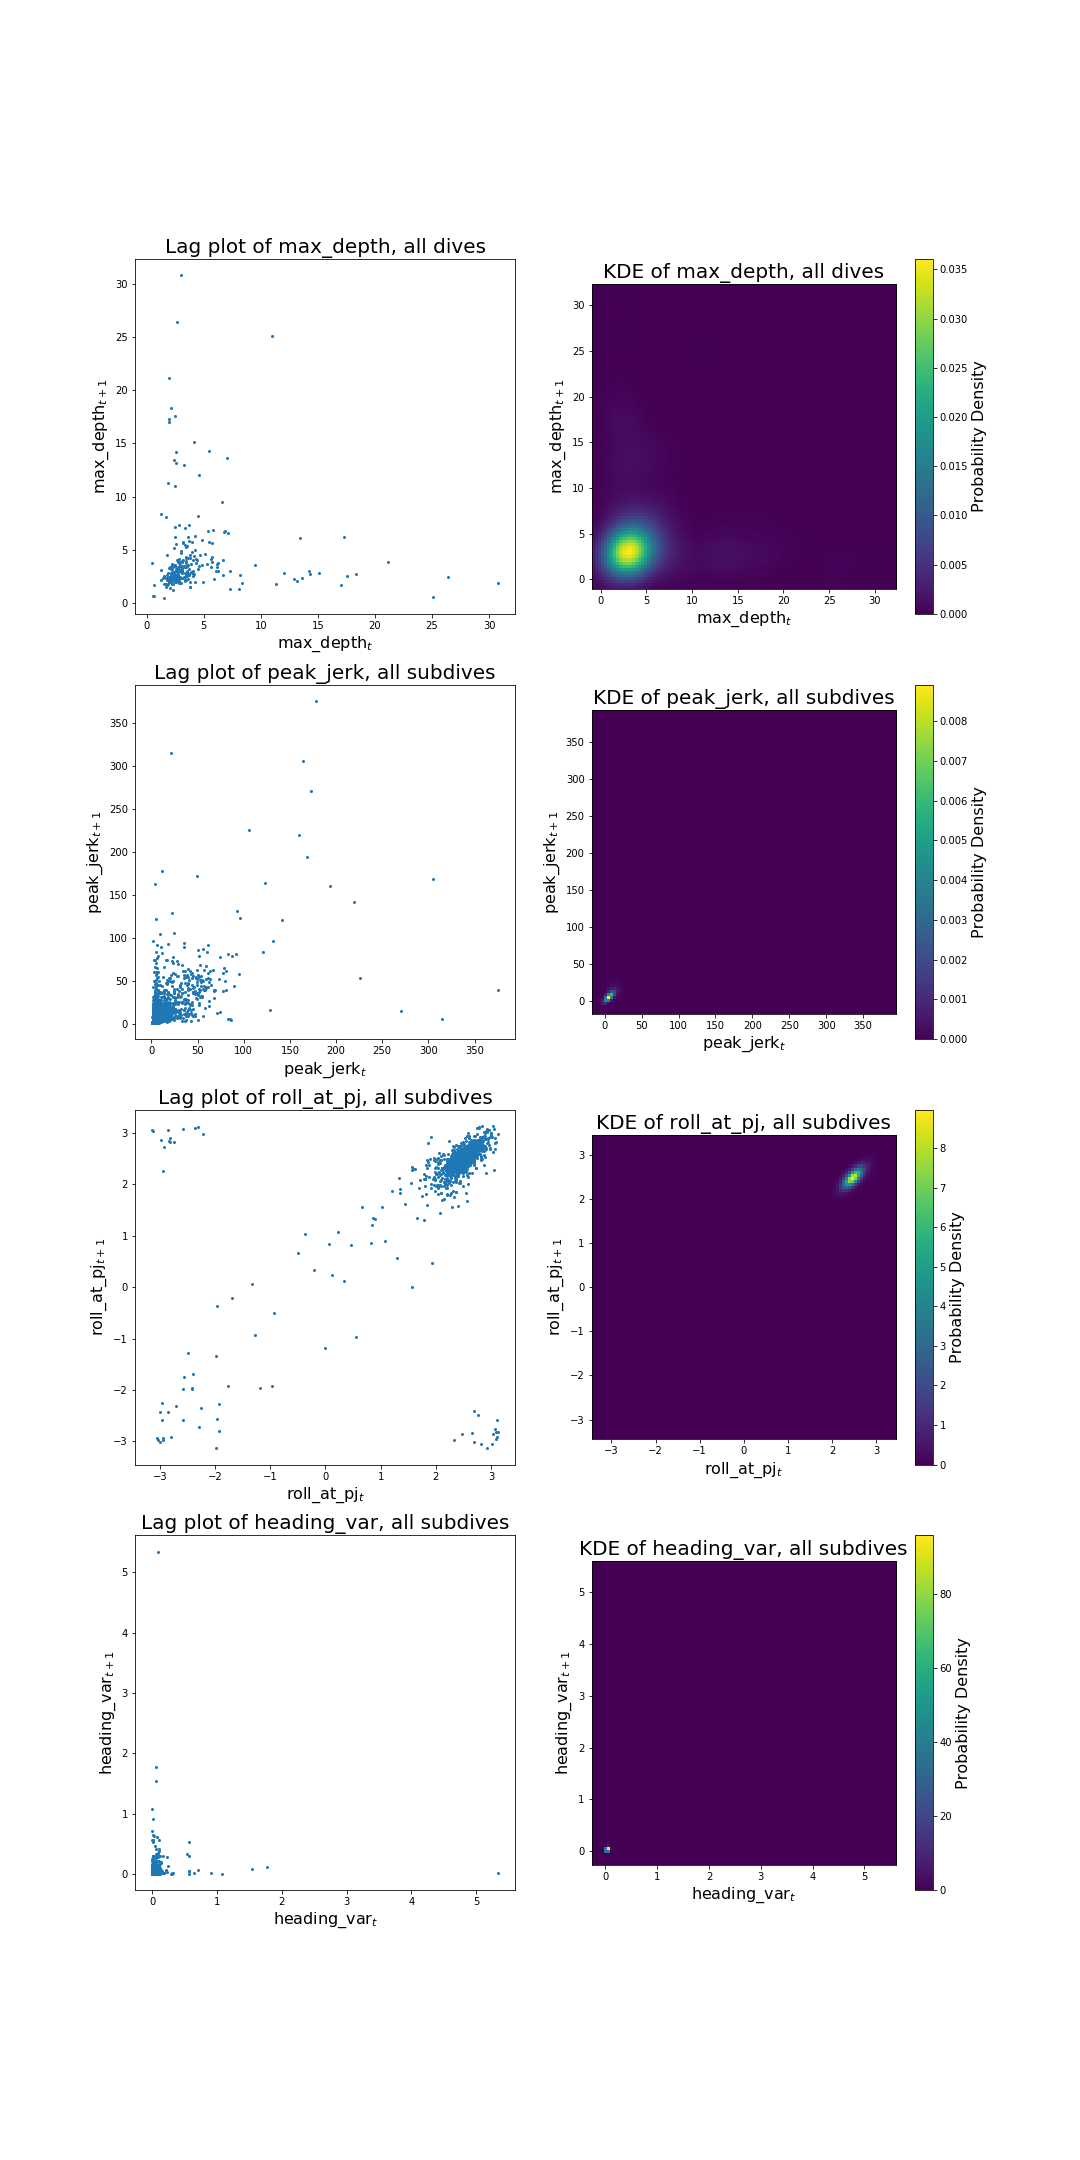
\includegraphics[height=5in]{../Plots/lagplot.png}
	\caption{Lag plot of vertical velocity and $\tilde a$ (left) and a the associated normal kernel density estimates (right)}
	\label{fig:data}
\end{figure}

\begin{figure}[h!]
	\centering
	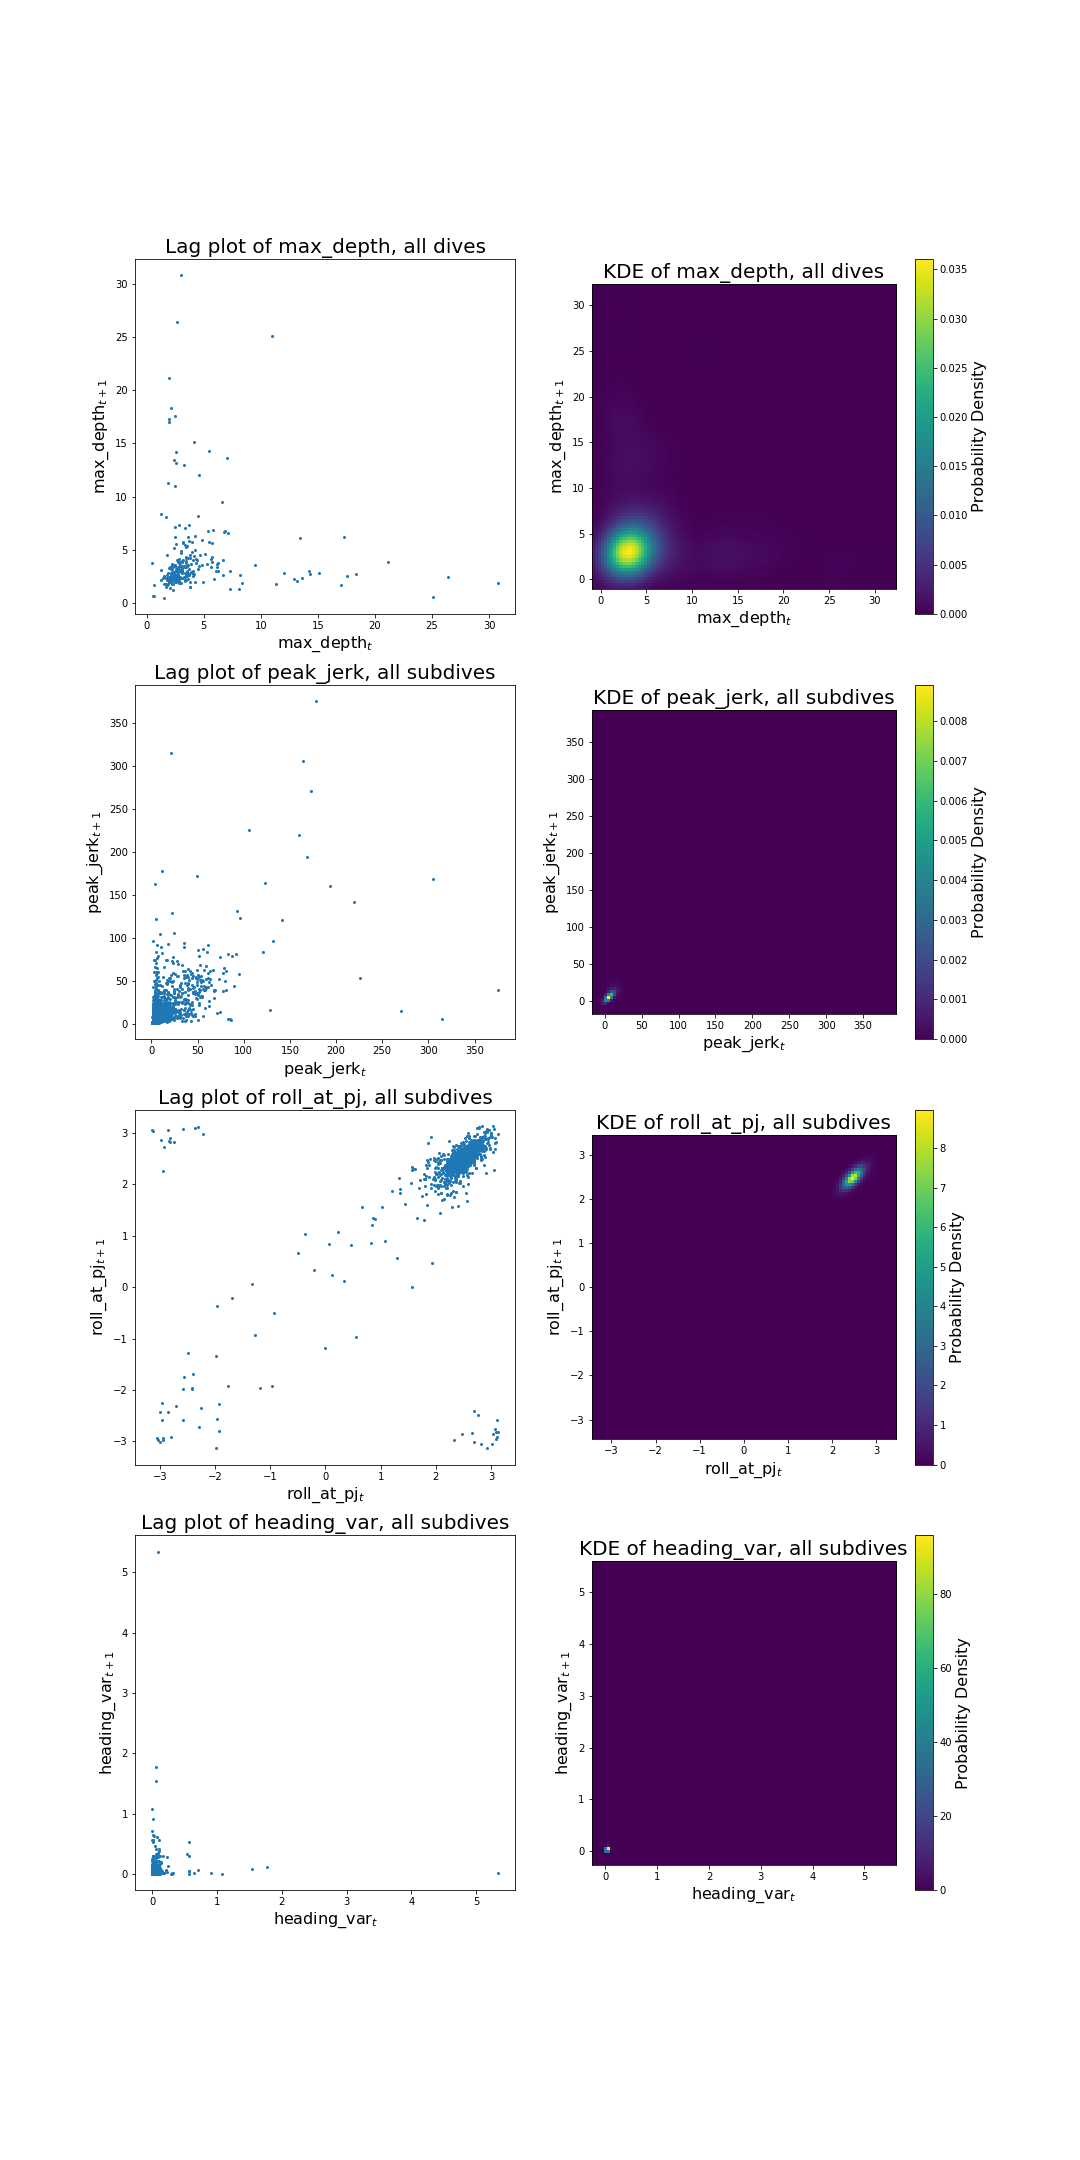
\includegraphics[height=5in]{../Plots/lagplot.png}
	\caption{Lag plot of vertical velocity and $\tilde a$ (left) and a the associated normal kernel density estimates (right)}
	\label{fig:data_one_dive}
\end{figure}

\subsection{Model Selection}

The collection of all dive durations were set to be the coarse-scale observations $Y$, and the acceleration data was used to determine the fine-scale observations $Y^*$. Figure (\ref{fig:raw_data_one_dive}) shows both the depth profile and the raw accelerometer data for one specific dive. The acceleration exhibits sinusoidal behavior at several points in time which cannot be modeled using HMMs without some kind of signal processing. Therefore, the STFT was used to calculate both $Y{*(1)}$ and $Y^{*(2)}$ as described in section \ref{subsec:STFT}. We set $\tilde{f} = 5$ hertz and $h = 2$ seconds, which reduced the dimension of each window from $50 s^{-1} * 2 s = 100$ to $2$.

In order to determine if the CarHHMM was appropriate for this data, a lag plot was made for both $Y^{*(1)}_{t,s^*}$ and $Y^{*(2)}_{t,s^*}$, as shown in figure (\ref{fig:lag}). The number of behavioral states is not clear from the lag plot, but it is clear that $Y^{*(1)}_{t,s^*}$ exhibits a large degree of auto-correlation. While $Y^{*(2)}_{t,s^*}$ also exhibits some auto-correlation, the relationship is less strong, so auto-correlation was not incorporated in the emission distribution of $Y^{*(2)}_{t,s^*}$. 

\begin{figure}[h!]
	\centering
	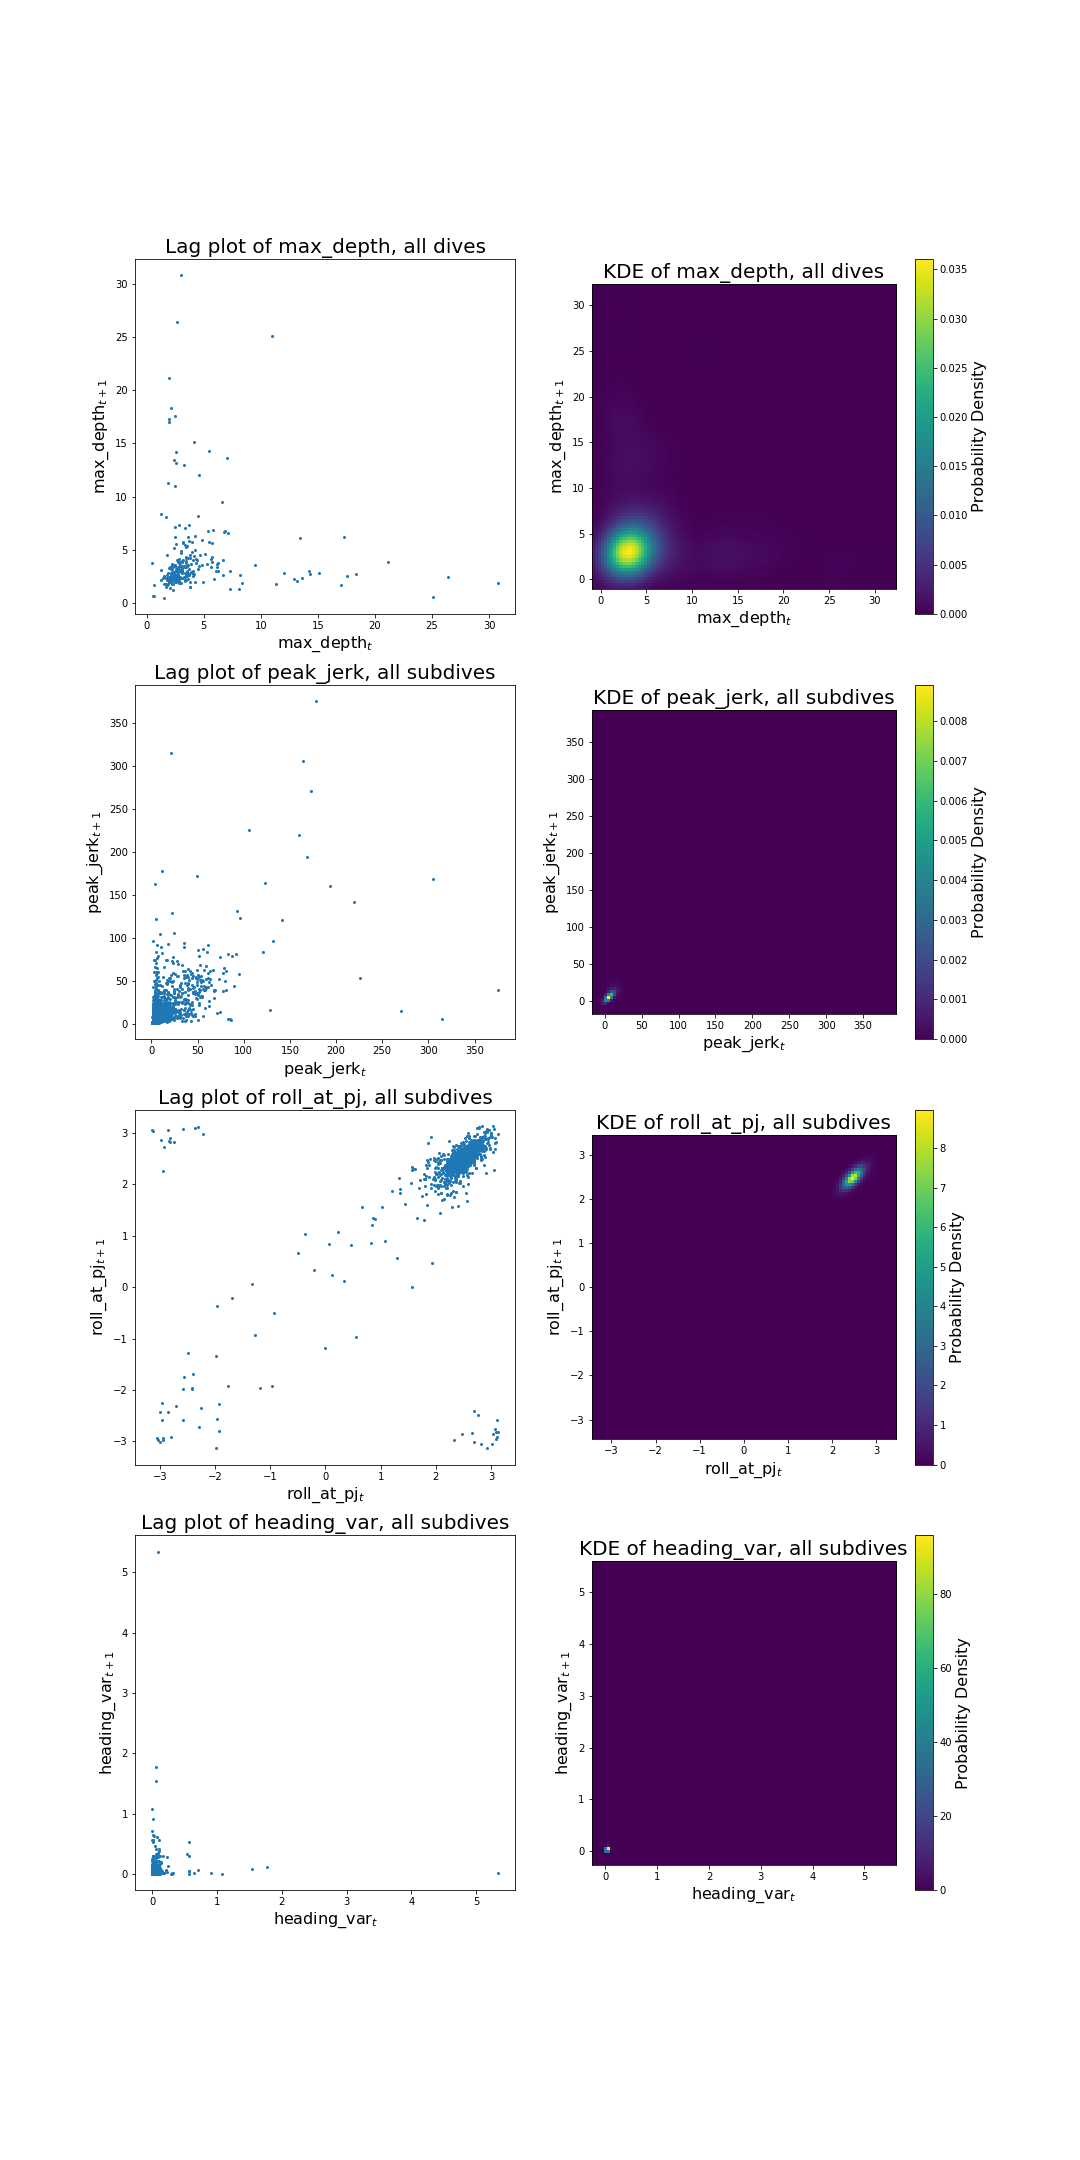
\includegraphics[height=5in]{../Plots/lagplot.png}
	\caption{Lag plot of vertical velocity and $\tilde a$ (left) and a the associated normal kernel density estimates (right)}
	\label{fig:lag}
\end{figure}

Information criteria tends to overestimate the number of states in biological processes \cite{Pohle:2017}, so we instead selected $N = 2$ dive types and $N^* = 3$ sub-dive behaviours heuristically and admittedly somewhat arbitrarily. This is a common issue in statistical ecology, so it is important to use model validation techniques in lieu of information criteria. Section \ref{subsec:model_validation} describes our process of validating this model in particular.

\subsection{Results}

The parameters of the estimated emission distributions for each behavioral state are shown in table (\ref{table:emis_dist}). Each distribution is also plotted in figures (\ref{fig:coarse_emis}) and (\ref{fig:fine_emis}). Note that the auto-correlation within the velocity sequence is not captured in figure (\ref{fig:emis_dist}), so it is important to refer to the estimated auto-correlation parameter $\hat \phi$ from table (\ref{table:emis_dists}) when considering the emission distributions shown in figure (\ref{fig:fine_emis}).
%
\begin{figure}[h!]
	\centering
	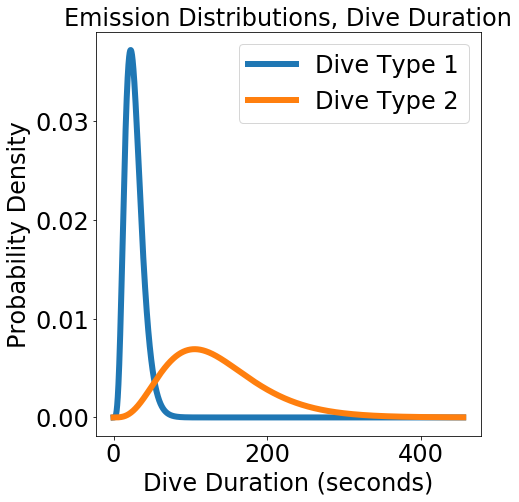
\includegraphics[height=4in]{../Plots/coarse-emissions.png}
	\caption{Estimated probability distributions for the long-term vertical velocity and $\tilde a$ in each behavioral state. Note that the distribution over vertical velocity does not take auto-correlation into account.}
	\label{fig:coarse_emis}
\end{figure}
%
\begin{figure}[h!]
	\centering
	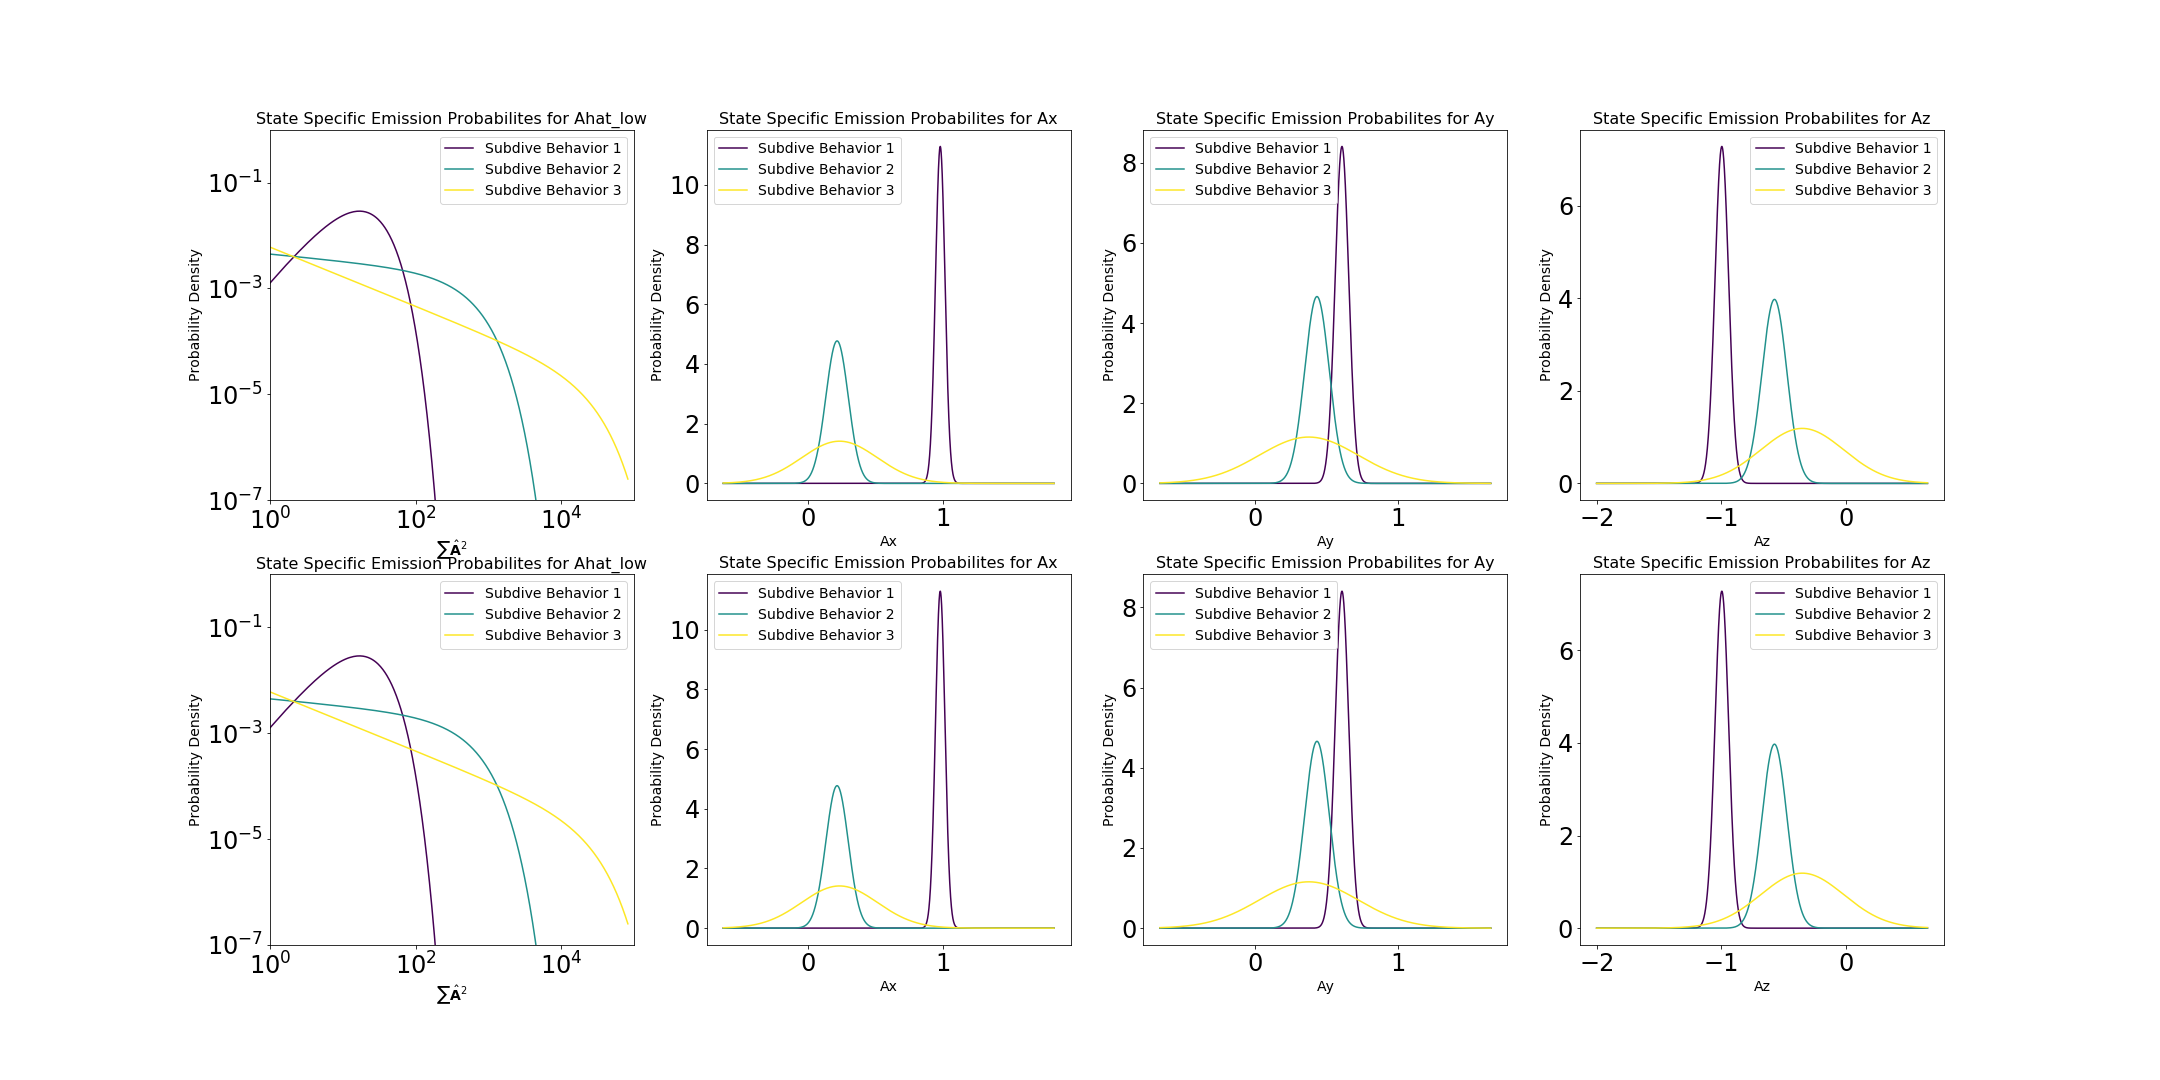
\includegraphics[height=2.5in]{../Plots/fine-emissions.png}
	\caption{Estimated probability distributions for the long-term vertical velocity and $\tilde a$ in each behavioral state. Note that the distribution over vertical velocity does not take auto-correlation into account.}
	\label{fig:coarse_emis}
\end{figure}
%
\begin{table}[h!]
    \centering
    \label{table:emis_dists}
    \caption{Estimates and standard errors of emission parameters for killer whale data.}
    \begin{tabular}{ccccc}
    \multirow{2}{*}{Feature}                 & \multirow{2}{*}{Dive / Subdive Type} & \multicolumn{3}{c}{Parameter Estimate}              \\
                                             &                                      & $\hat \mu$      & $\hat \sigma$   & $\hat \phi$     \\ \hline
    \multirow{2}{*}{Dive Duration (seconds)} & 1                                    & $27.23 \pm 0.63$ & $10.89 \pm 0.56$ & ---             \\
                                             & 2                                    & $127.96 \pm 11.50$ & $64.13 \pm 9.21$ & ---             \\ \hline
    \multirow{3}{*}{$Y^{*(1)}_x$}            & 1                                    & $0.98 \pm 0.07$ & $0.04 \pm 0.00$ & $0.99 \pm 0.00$ \\
                                             & 2                                    & $0.22 \pm 0.01$ & $0.08 \pm 0.00$ & $0.87 \pm 0.01$ \\
                                             & 3                                    & $0.23 \pm 0.03$ & $0.28 \pm 0.01$ & $0.62 \pm 0.03$ \\ \hline
    \multirow{3}{*}{$Y^{*(1)}_y$}            & 1                                    & $0.61 \pm 0.09$ & $0.05 \pm 0.00$ & $0.99 \pm 0.00$ \\
                                             & 2                                    & $0.43 \pm 0.01$ & $0.09 \pm 0.00$ & $0.87 \pm 0.01$ \\
                                             & 3                                    & $0.38 \pm 0.04$ & $0.35 \pm 0.01$ & $0.62 \pm 0.04$ \\ \hline
    \multirow{3}{*}{$Y^{*(1)}_z$}            & 1                                    & $-1.00 \pm 0.11$ & $0.05 \pm 0.00$ & $0.99 \pm 0.00$ \\
                                             & 2                                    & $-0.57 \pm 0.01$ & $0.10 \pm 0.00$ & $0.87 \pm 0.01$ \\
                                             & 3                                    & $-0.35 \pm 0.04$ & $0.34 \pm 0.01$ & $0.62 \pm 0.04$ \\ \hline
    \multirow{3}{*}{$Y^{*(2)}$}              & 1                                    & $27.16 \pm 0.32$ & $16.67 \pm 0.32$ & ---             \\
                                             & 2                                    & $406.98 \pm 4.42$ & $438.09 \pm 5.49$ & ---             \\
                                             & 3                                    & $9688.54 \pm 221.95$ & $14584.02 \pm 358.40$ & ---             \\ \hline
    \end{tabular}
\end{table}
%
While the ecological meaning of these behavioral states is tenuous, we hypothesize the following interpretations. For the coarse-scale, dive type 1 corresponds to shorter, shallower dives that the killer whale uses to rest before performing a dive of type 2, which corresponds to a deeper, more sustained dive. For the fine-scale, behavioral state 1 corresponds to gliding and passive swimming. The mean of $Y^{*(2)}$ in this state is at least an order of magnitude smaller than sub-dive behavior 2, the variance of $Y^{*(1)}$ is smaller, and the autocorrelation of $Y^{*(1)}$ is higher than every other behavioral state.  This indicates a relatively constant reading of acceleration and therefore low levels of activity. On the other hand, sub-dive state 3 corresponds to vigorous swimming activity, as the mean of $Y^{*(2)}$ and variance of $Y^{*(1)}$ are much higher than every other state. The auto-correlation of $Y^{*(1)}$ is also much lower in this state, implying more variation in acceleration every 2 seconds. Behavioral state 2 is between the other two behavioral states in almost every parameter estimate.
The estimated probability transition matrices and associated stationary distributions are shown below:
%
$$\hat \Gamma = \begin{pmatrix} 
0.849 & 0.151 \\
0.907 & 0.093
\end{pmatrix}$$
$$\hat \delta = \begin{pmatrix} 0.857 & 0.143 \end{pmatrix}$$
%
$$\hat \Gamma^{*(1)} = \begin{pmatrix} 
0.724 & 0.276 & 0.000 \\
0.057 & 0.887 & 0.056 \\
0.000 & 0.247 & 0.753
\end{pmatrix} \qquad 
\hat \Gamma^{*(2)} = \begin{pmatrix} 
0.871 & 0.129 & 0.000 \\
0.135 & 0.829 & 0.036 \\
0.000 & 0.246 & 0.754
\end{pmatrix}$$
$$\hat \delta^{*(1)} = \begin{pmatrix} 0.143 & 0.698 & 0.159 \end{pmatrix} \qquad
\hat \delta^{*(2)} = \begin{pmatrix} 0.476 & 0.456 & 0.067 \end{pmatrix}$$
%
About 85\% of the dives observed here are short, as the whale usually rests for many dives in a row before performing a deep dive. Interestingly, the probability transition matrix $\hat \Gamma$ shows that the current dive does not effect the dive type of the following dive much. In addition, the fine-scale probability transition matrices imply that the killer whale is much more likely to be in a less active sub-dive state when performing deep dives than when performing shallow dives- 14\% of shallow dives are spend in sub-dive state 1 while 48\% of deep dives are spent in sub-dive state 1. This is likely because the killer whale needs to conserve energy when diving at depth and holding its breath for longer.

Finally, the decoded dive behavior within a selected dive (deeper than 20 meters) is shown in figure (\ref{fig:labeled_dives}). In addition, the probability of each dive type and sub-dive state is shown in (fig \ref{fig:coarse_probs}) and (fig \ref{fine_probs}), respectively.

\begin{figure}[h!]
	\centering
	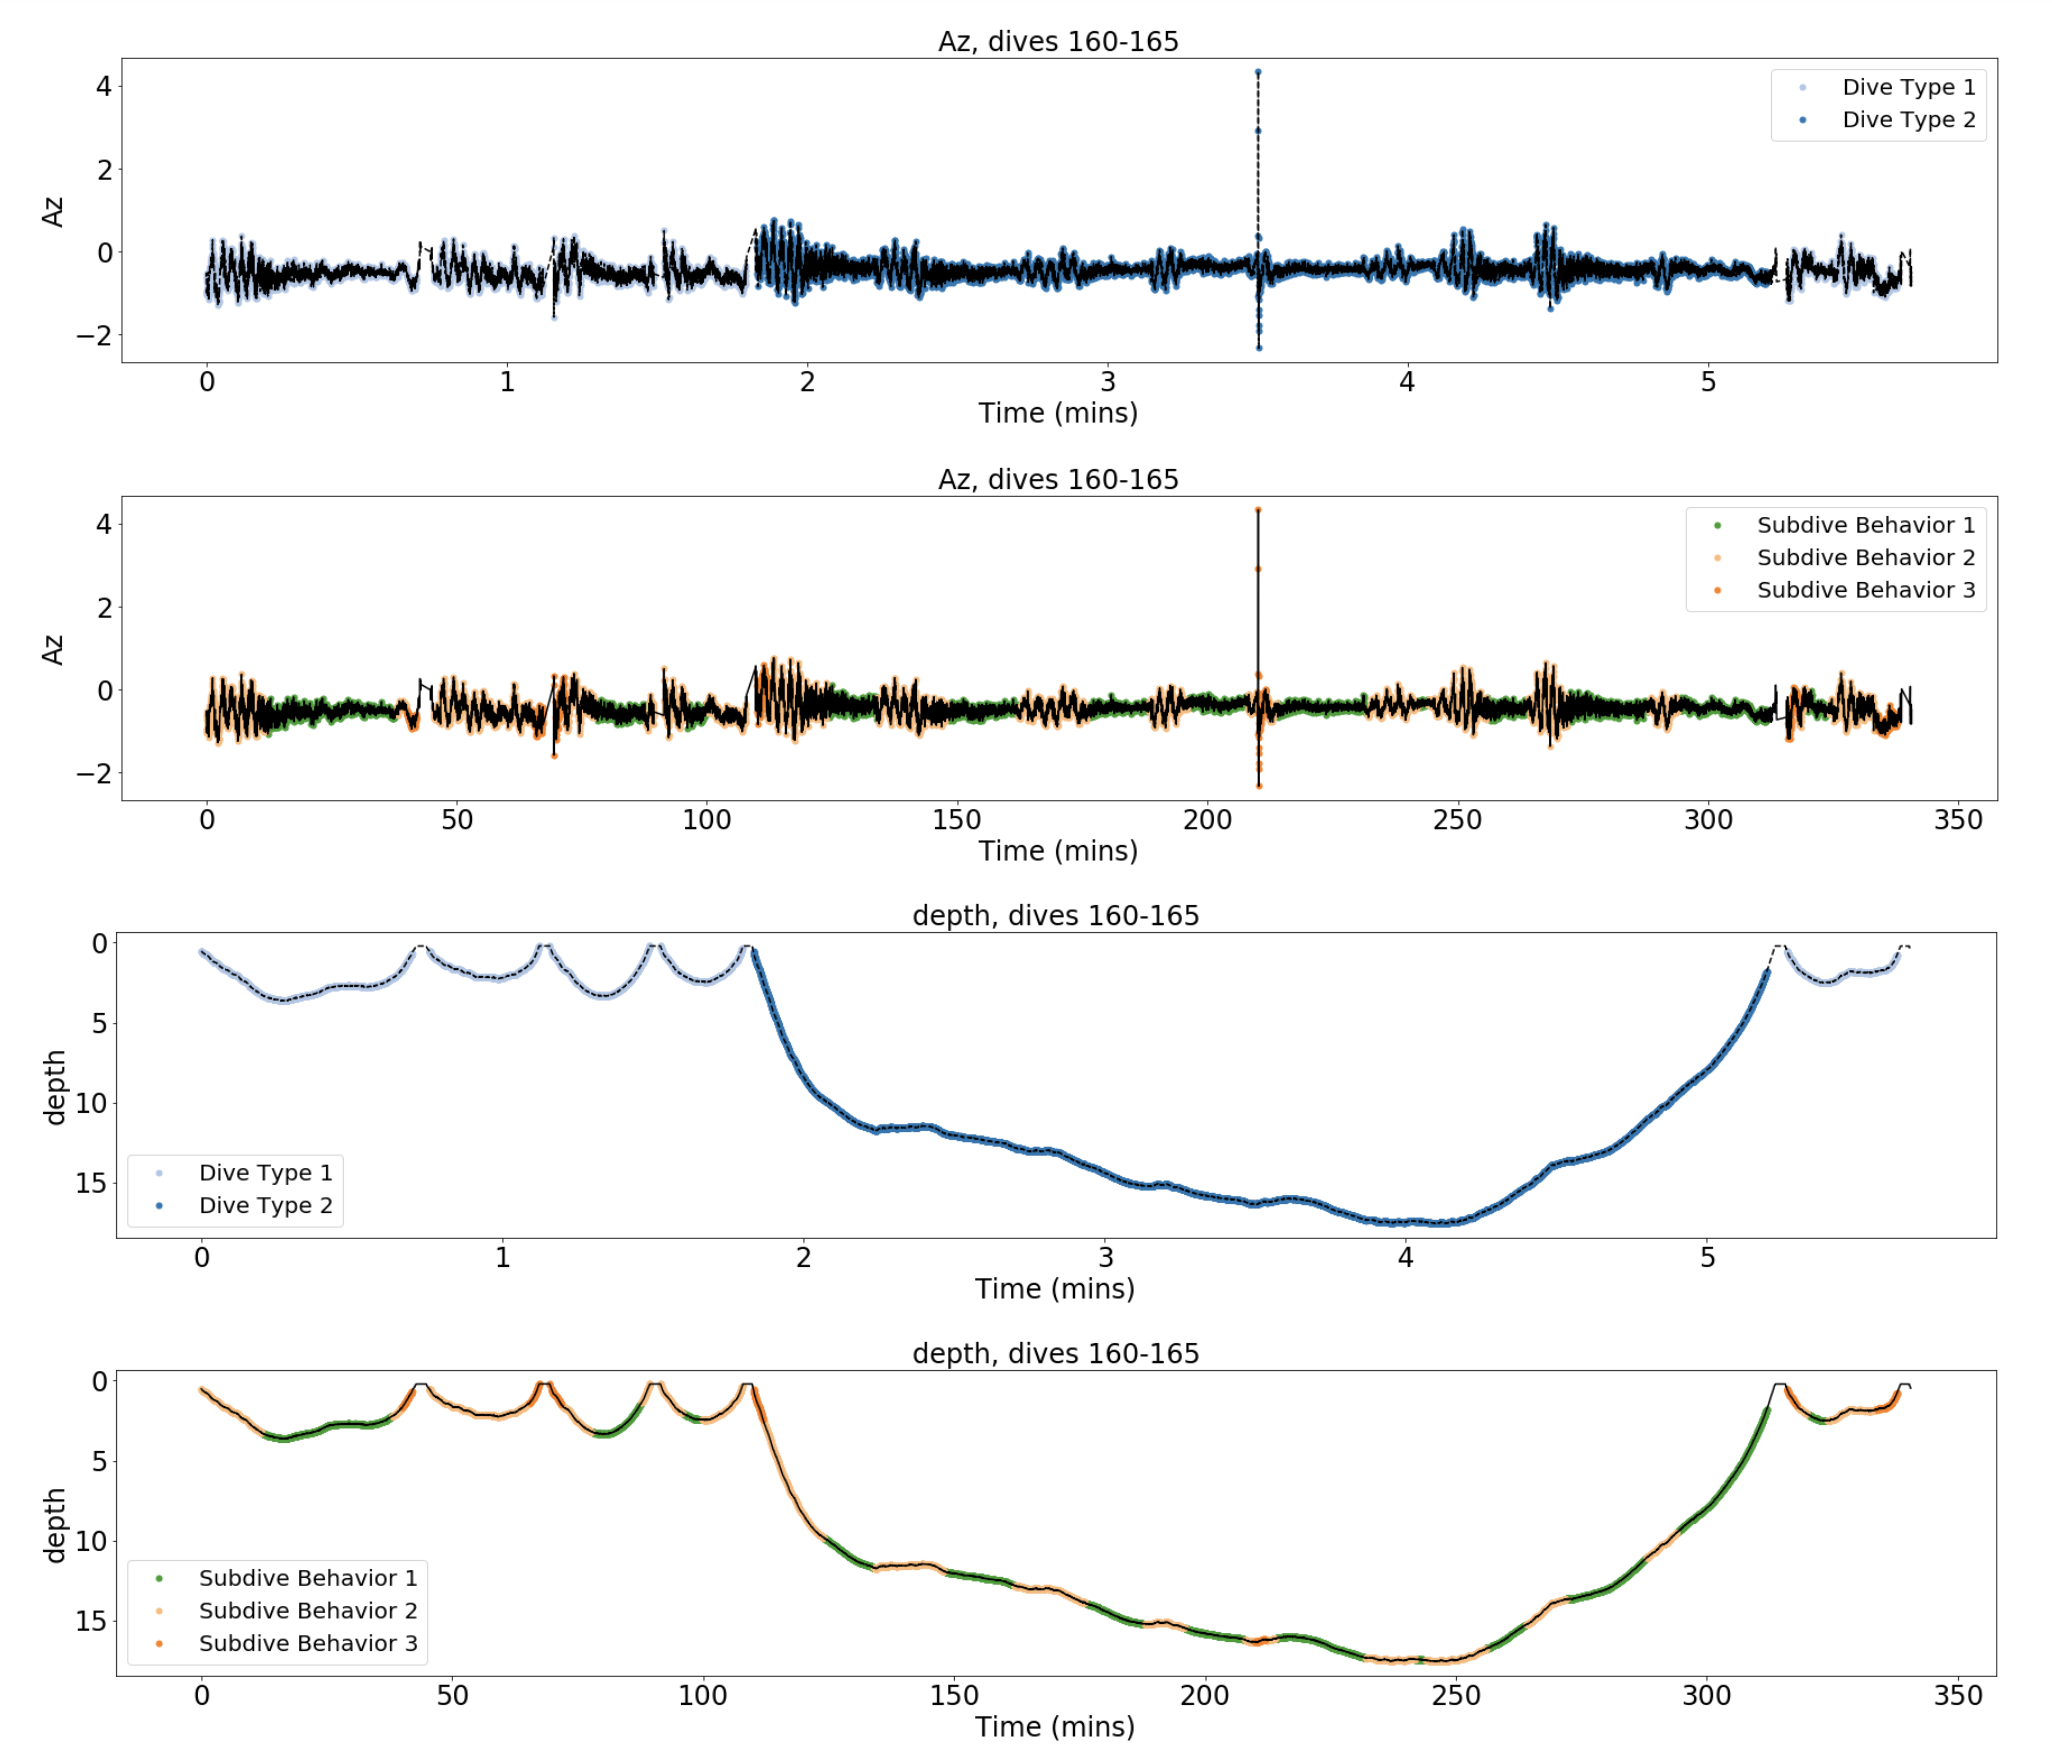
\includegraphics[width=5in]{../Plots/labeled_dives.png}
	\caption{Features of a particular set of killer whale dives and Viterbi-decoded estimates for the intra-dive behavioral states.}
	\label{fig:labeled_dives}
\end{figure}
%
\begin{figure}[h!]
	\centering
	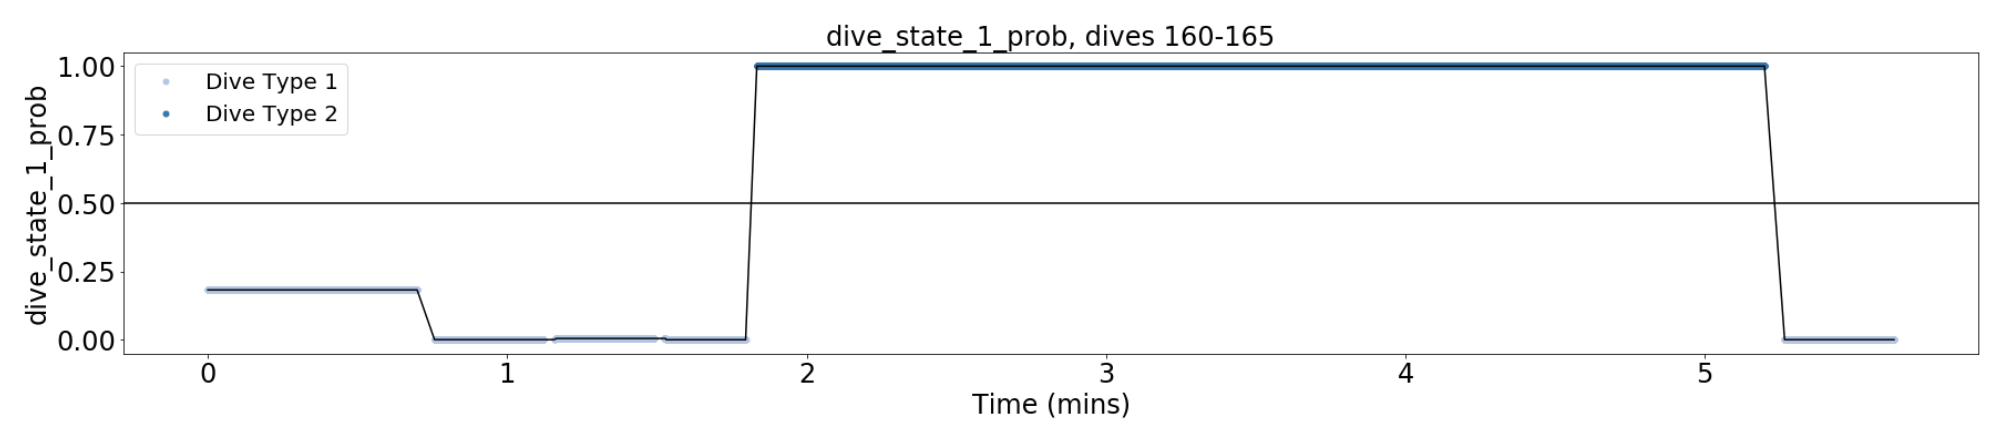
\includegraphics[width=5in]{../Plots/Coarse_state_probs.png}
	\caption{Probability of dive types for a particular set of killer whale dives.}
	\label{fig:coarse_probs}
\end{figure}
%
\begin{figure}[h!]
	\centering
	\begin{subfigure}[t]{1.0\textwidth}
        \centering
        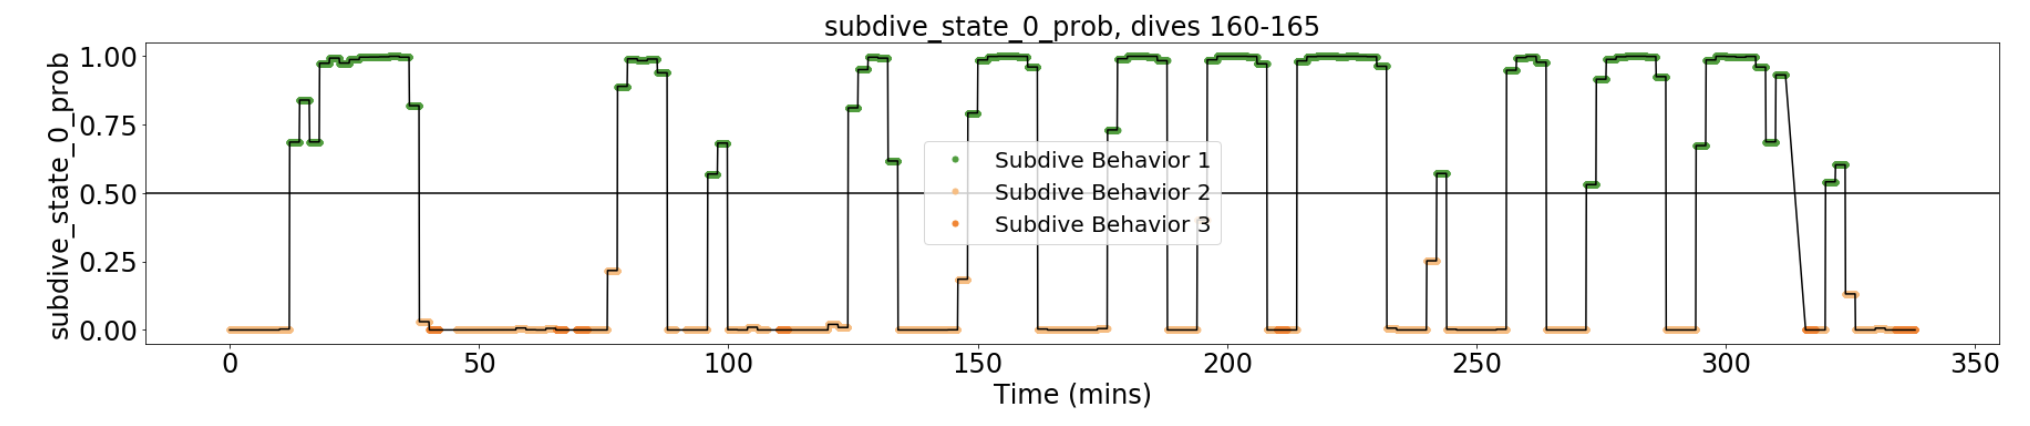
\includegraphics[width=5in]{../Plots/Fine_state_probs_1.png}
        \caption{Fine-scale state 1 probabilities}
    \end{subfigure}
    \newline
    \begin{subfigure}[t]{1.0\textwidth}
        \centering
        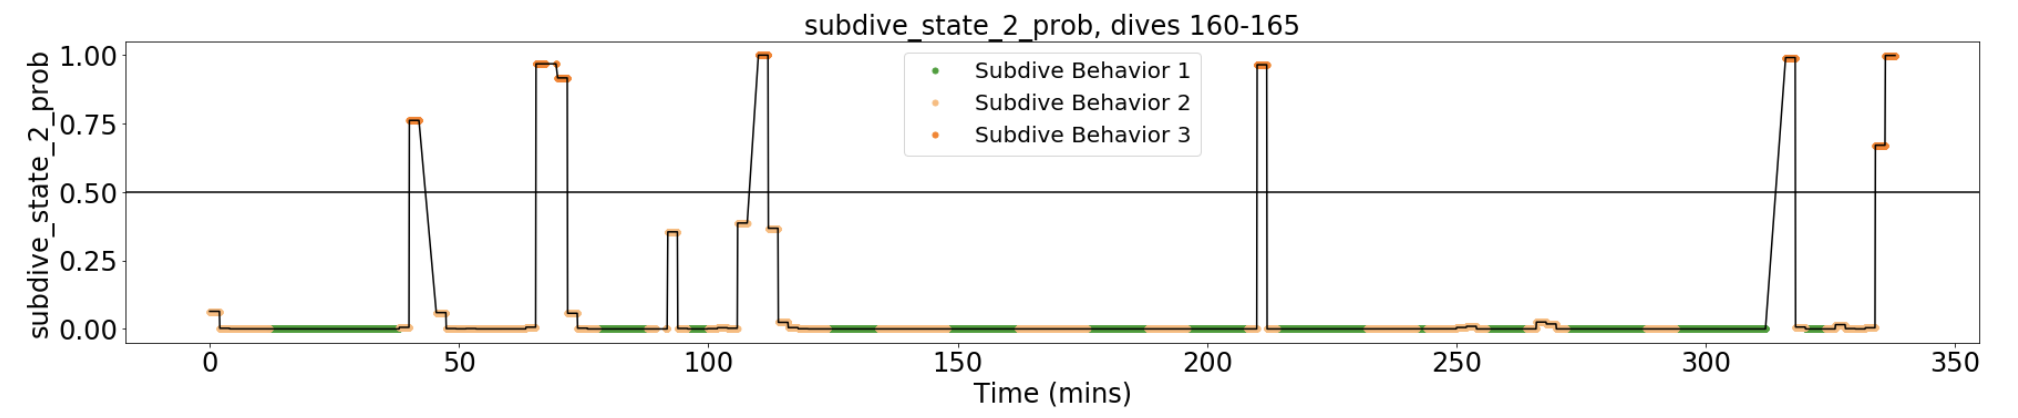
\includegraphics[width=5in]{../Plots/Fine_state_probs_3.png}
        \caption{Fine-scale state 3 probabilities}
    \end{subfigure}
	\caption{Probability of sub-dive types for a particular set of killer whale dives.}
	\label{fig:fine_probs}
\end{figure}

\subsection{Model Validation}
\label{model_validation}

Two visual tools were used to evaluate the model for this data: pseudo-residuals and empirical histograms. A pseudo-residual of a particular observation, as described in \cite{Zucchini:2016}, is the marginal cdf of an observation, conditioned on all other observations, and mapped to the quantile function of a standard normal distribution. In particular, the pseudo-residual of an observation $y_{t,s^*}$ is $\Phi^{-1} \left(Pr(Y_{t,s^*} < y_{t,s^*}|Y/Y_{t,s^*}) \right)$, where $\Phi$ is the cdf of a standard normal distribution. If the model is well-specified, then all pseudoresiduals should be independent and follow a standard normal distribution. While histograms of the pseudoresiduals support this for all features, one notable exception is the case of $Y^{*(2)}$, shown in (fig \ref{fig:pseudoresids}). These psuedoresiduals are noticeably right-skewed, implying that the true distribution of $Y^{*(2)}$ may follow a heavier-tailed distribution compared to a gamma distribution such as a power law. 

\begin{figure}[h!]
	\centering
	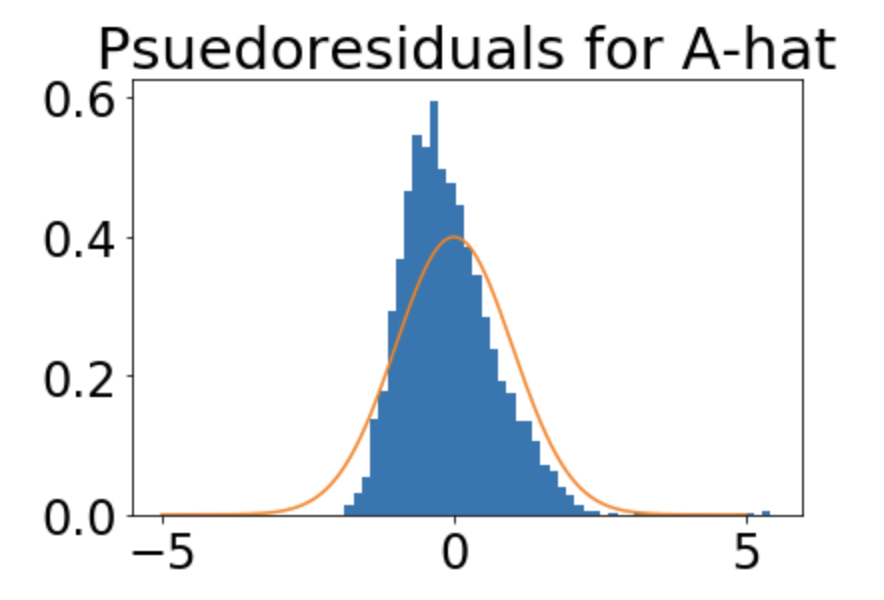
\includegraphics[width=5.5in]{../Plots/pseudoresids.png}
	\caption{Psuedoresiduals of $Y^{*(2)}$}
	\label{fig:pseudoresids}
\end{figure}

In addition to psuedoresiduals, we plotted a histogram of observations for each feature where the observations were weighted by the probability that the whale was in a particular hidden state. This empirical distribution was then be plotted on top of the estimated true pdf of that feature conditioned on the hidden state. This procedure is similar to that for pseudo-residuals, but it produces individual plots for each sub-dive state. Again, our results mostly support the model in question with the exception of $Y^{*(2)}$, which is right-skewed. In addition, $Y^{*(1)}$ has heavy tails for sub-dive state 3 (see fig \ref{fig:empirical_dist}), indicating the existence of rare events corresponding to very violent trashing of the killer whale. These outliers are potential subjects for future studies to better understand rare behavioral events for this killer whale.

\begin{figure}[h!]
	\centering
	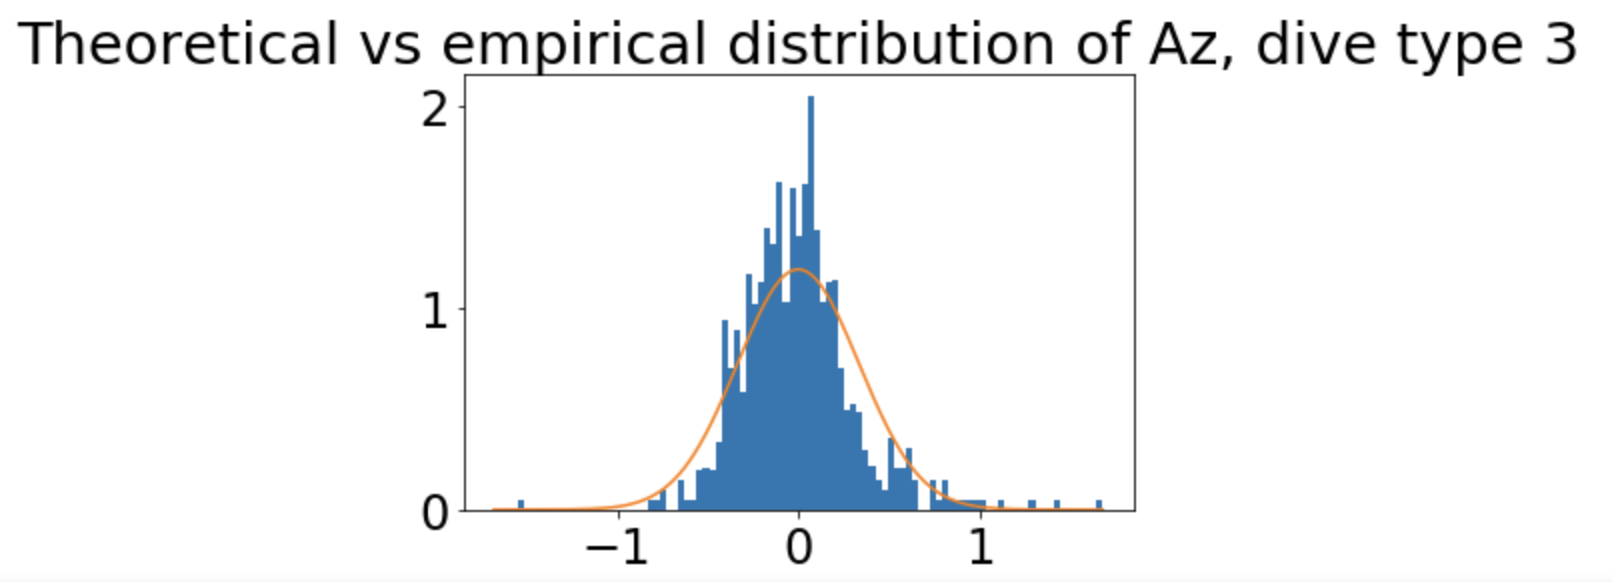
\includegraphics[width=5.5in]{../Plots/empirical_dist.png}
	\caption{Empirical Distribution of $Y^{*(1)}_z$ for sub-dive state 3 plotted against its estimated pdf}
	\label{fig:empirical_dist}
\end{figure}